% 原书第189—191页；9.5.3、9.5.4。
\subsection{基于协方差的约束}
另一类约束出现在含潜变量的线性模型中。例如，对图9.8，可以得到以下\textbf{四元约束（tetrad constraint）}［Spirtes et al., 2000；Spearman, 1904］：
\begin{equation}
 \rho_{AC}\rho_{BD}-\rho_{AD}\rho_{BC}=0,\tag{9.12}
\end{equation}
\begin{equation}
 \rho_{AB}\rho_{CD}-\rho_{AD}\rho_{BC}=0,\tag{9.13}
\end{equation}
\begin{equation}
 \rho_{AC}\rho_{BD}-\rho_{AB}\rho_{CD}=0,\tag{9.14}
\end{equation}
其中$\rho_{AC}$是变量$A$与$C$的相关系数。\chninenote{图9.8实际含有两个潜在因子及箭头$H\to J$。一般线性结构因果模型中，式(9.12)成立，但式(9.13)、(9.14)还需要额外条件。若$J:=\eta H+N_J$，则$\Cov(A,B)\Cov(C,D)-\Cov(A,D)\Cov(B,C)=\alpha\beta\gamma\delta\Var(H)\Var(N_J)$，通常不为零；例如再要求$\Var(N_J)=0$才可消去这一项。原图、图注及三条编号公式均予保留。}例如，第一条约束(9.12)可以很容易地从图9.8验证：
\[
\begin{aligned}
 \Cov(A,C)\cdot\Cov(B,D)
 &=\alpha\gamma\eta\Var(H)\cdot\beta\delta\eta\Var(H)\\
 &=\alpha\delta\eta\Var(H)\cdot\beta\gamma\eta\Var(H)
 =\Cov(A,D)\cdot\Cov(B,C).
\end{aligned}
\]
\begin{figure}[htbp]
\centering
\begin{tikzpicture}[causal,x=1.5cm,y=1.2cm]
 \node[latent] (ch09f8-h) at (.75,1) {$H$};
 \node[latent] (ch09f8-j) at (3,1) {$J$};
 \node[vtx] (ch09f8-a) at (0,0) {$A$};
 \node[vtx] (ch09f8-b) at (1.5,0) {$B$};
 \node[vtx] (ch09f8-c) at (2.25,0) {$C$};
 \node[vtx] (ch09f8-d) at (3.75,0) {$D$};
 \draw[ed] (ch09f8-h)--node[left] {$\alpha$}(ch09f8-a);
 \draw[ed] (ch09f8-h)--node[below left] {$\beta$}(ch09f8-b);
 \draw[ed] (ch09f8-h)--node[above] {$\eta$}(ch09f8-j);
 \draw[ed] (ch09f8-j)--node[below right] {$\gamma$}(ch09f8-c);
 \draw[ed] (ch09f8-j)--node[right] {$\delta$}(ch09f8-d);
\end{tikzpicture}
\caption{如果该图对应一个线性结构因果模型，其导出的分布将满足四元约束(9.12)—(9.14)。}
\end{figure}


可以利用\textbf{无对撞路径（trek）}与\textbf{瓶颈点（choke point）}的语言，以图形方式刻画四元约束何时为零［Spirtes et al., 2000，定理6.10］。这些约束同样使我们仅凭观测数据，就能区分不同因果结构。Bollen［1989］与Wishart［1928］构造了检验四元差是否为零的统计检验。还可以将这些检验转化为因果学习所用的得分；例如Spirtes et al.［2000，第11.2节］与Silva et al.［2006］对此进行了研究。

Kela et al.［2017］考察这样一类潜变量结构：观测变量之间的一切相依关系，都源于一组相互独立的共同原因。他们描述了观测变量可能具有的协方差矩阵所受的约束，并强调，与使用完整分布相比，转而使用协方差矩阵，在统计可行性与计算可处理性方面都具有优势。通过采用观测变量的函数，即像基于再生核Hilbert空间的方法那样将变量映射到特征空间，该方法也能考虑高阶相依关系。

\subsection{加性噪声模型}
第7.2.3节已经提到，可以利用独立成分分析（ICA）来学习线性非高斯无环模型（LiNGAM）的结构。Hoyer et al.［2008b］说明，借助所谓的\textbf{过完备独立成分分析（overcomplete ICA）}，可以将可识别性结论与相应方法推广到含潜变量的线性非高斯结构。

对于非线性加性噪声模型（ANM，见第4.1.4节），我们已经看到，在一般情形下，不可能同时有$Y=f(X)+N_Y$、$N_Y\indep X$，以及$X=g(Y)+M_X$、$M_X\indep Y$。我们预期，对潜变量也存在类似的可识别性。下面的加性噪声模型描述潜变量$H$对可观测变量$X,Y$的影响：
\begin{equation}
 H:=N_H,\tag{9.15}
\end{equation}
\begin{equation}
 X:=f(H)+N_X,\tag{9.16}
\end{equation}
\begin{equation}
 Y:=g(H)+N_Y.\tag{9.17}
\end{equation}

在噪声足够低的情形下，Janzing et al.［2009a］证明，可以从$P_{X,Y}$重建联合分布$P_{H,X,Y}$，至多相差对$H$的重参数化。低噪声的限制可能并非必要，而只是证明本身的不足。令$f(H)=H$、$N_X=0$，就得到从$X$到$Y$的加性噪声模型；同样，也可以得到从$Y$到$X$的模型。这提示，加性噪声假设可能使我们仅凭$P_{X,Y}$，就能区分$X\to Y$、$X\leftarrow Y$与$X\leftarrow *\to Y$这三种情况。

这一模型与降维之间的联系，有助于理解如何根据数据拟合模型(9.15)—(9.17)：可以按照以下步骤，从分布$P_{X,Y}$抽取数据点$(x,y)$，见图9.9。
\begin{enumerate}[label=\arabic*.]
 \item 按$P_H$抽取$h$。
 \item 考虑流形
 \begin{equation}
 M:=\bigl\{\bigl(f(h),g(h)\bigr)\in\mathbb R^2:h\in\mathbb R\bigr\}
 \tag{9.18}
 \end{equation}
 上对应的点$\bigl(f(h),g(h)\bigr)$。
 \item 在各个维度上加入相互独立的噪声$(n_X,n_Y)$。
\end{enumerate}
\begin{figure}[htbp]
\centering
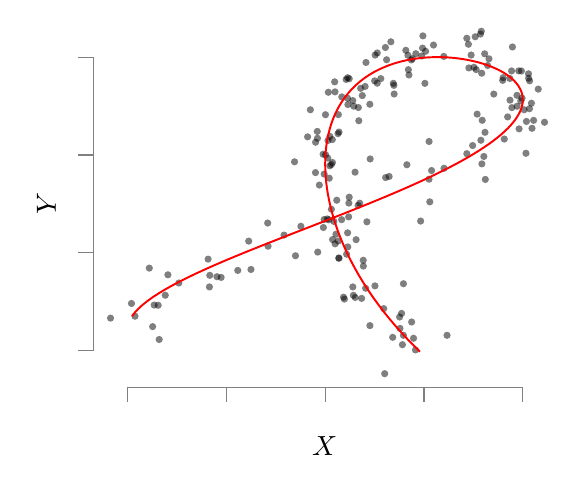
\begin{tikzpicture}[x=.035cm,y=.035cm]
\draw[gray,line width=.4pt] (20.483673,13.155319)--(163.857849,13.155319);
\draw[gray,line width=.4pt] (20.483673,13.155319)--(20.483673,7.775436);
\draw[gray,line width=.4pt] (56.319748,13.155319)--(56.319748,7.775436);
\draw[gray,line width=.4pt] (92.165771,13.155319)--(92.165771,7.775436);
\draw[gray,line width=.4pt] (128.011841,13.155319)--(128.011841,7.775436);
\draw[gray,line width=.4pt] (163.857849,13.155319)--(163.857849,7.775436);
\draw[gray,line width=.4pt] (7.990341,26.435699)--(7.990341,132.977554);
\draw[gray,line width=.4pt] (7.990341,26.435699)--(2.610458,26.435699);
\draw[gray,line width=.4pt] (7.990341,61.952972)--(2.610458,61.952972);
\draw[gray,line width=.4pt] (7.990341,97.470245)--(2.610458,97.470245);
\draw[gray,line width=.4pt] (7.990341,132.977554)--(2.610458,132.977554);
\fill[black,opacity=.5] (30.127609,43.023712) circle[radius=1.3pt];
\fill[black,opacity=.5] (14.286804,38.291397) circle[radius=1.3pt];
\fill[black,opacity=.5] (21.888397,43.601547) circle[radius=1.3pt];
\fill[black,opacity=.5] (23.163635,38.978821) circle[radius=1.3pt];
\fill[black,opacity=.5] (31.930862,30.540359) circle[radius=1.3pt];
\fill[black,opacity=.5] (29.569687,35.202942) circle[radius=1.3pt];
\fill[black,opacity=.5] (31.572205,42.953964) circle[radius=1.3pt];
\fill[black,opacity=.5] (28.354225,56.433594) circle[radius=1.3pt];
\fill[black,opacity=.5] (35.099030,54.002663) circle[radius=1.3pt];
\fill[black,opacity=.5] (39.074173,51.023819) circle[radius=1.3pt];
\fill[black,opacity=.5] (34.142593,46.590378) circle[radius=1.3pt];
\fill[black,opacity=.5] (50.302216,53.813385) circle[radius=1.3pt];
\fill[black,opacity=.5] (50.162735,49.609116) circle[radius=1.3pt];
\fill[black,opacity=.5] (54.416840,53.056213) circle[radius=1.3pt];
\fill[black,opacity=.5] (49.684525,59.691429) circle[radius=1.3pt];
\fill[black,opacity=.5] (52.892525,53.315247) circle[radius=1.3pt];
\fill[black,opacity=.5] (60.454262,55.596718) circle[radius=1.3pt];
\fill[black,opacity=.5] (65.236404,55.945412) circle[radius=1.3pt];
\fill[black,opacity=.5] (77.241547,68.408844) circle[radius=1.3pt];
\fill[black,opacity=.5] (64.419449,66.217041) circle[radius=1.3pt];
\fill[black,opacity=.5] (71.443207,64.373917) circle[radius=1.3pt];
\fill[black,opacity=.5] (71.303719,72.782501) circle[radius=1.3pt];
\fill[black,opacity=.5] (81.396019,60.916840) circle[radius=1.3pt];
\fill[black,opacity=.5] (95.762329,65.240677) circle[radius=1.3pt];
\fill[black,opacity=.5] (98.143433,74.007912) circle[radius=1.3pt];
\fill[black,opacity=.5] (91.787170,74.067688) circle[radius=1.3pt];
\fill[black,opacity=.5] (91.508240,71.168533) circle[radius=1.3pt];
\fill[black,opacity=.5] (104.111145,79.158661) circle[radius=1.3pt];
\fill[black,opacity=.5] (104.688965,79.985588) circle[radius=1.3pt];
\fill[black,opacity=.5] (100.883179,82.167419) circle[radius=1.3pt];
\fill[black,opacity=.5] (107.299210,73.220879) circle[radius=1.3pt];
\fill[black,opacity=.5] (121.804993,93.933456) circle[radius=1.3pt];
\fill[black,opacity=.5] (114.093811,89.290802) circle[radius=1.3pt];
\fill[black,opacity=.5] (115.369049,89.679352) circle[radius=1.3pt];
\fill[black,opacity=.5] (130.123917,80.473755) circle[radius=1.3pt];
\fill[black,opacity=.5] (130.761536,91.831322) circle[radius=1.3pt];
\fill[black,opacity=.5] (126.796326,73.499817) circle[radius=1.3pt];
\fill[black,opacity=.5] (129.834991,88.693039) circle[radius=1.3pt];
\fill[black,opacity=.5] (135.284622,92.658218) circle[radius=1.3pt];
\fill[black,opacity=.5] (143.553711,97.948456) circle[radius=1.3pt];
\fill[black,opacity=.5] (129.864868,102.371918) circle[radius=1.3pt];
\fill[black,opacity=.5] (150.268616,88.603378) circle[radius=1.3pt];
\fill[black,opacity=.5] (149.730652,96.942223) circle[radius=1.3pt];
\fill[black,opacity=.5] (148.654663,102.820244) circle[radius=1.3pt];
\fill[black,opacity=.5] (149.142838,110.063179) circle[radius=1.3pt];
\fill[black,opacity=.5] (149.013306,94.252274) circle[radius=1.3pt];
\fill[black,opacity=.5] (150.149078,105.689526) circle[radius=1.3pt];
\fill[black,opacity=.5] (147.299744,112.294846) circle[radius=1.3pt];
\fill[black,opacity=.5] (162.512878,106.954803) circle[radius=1.3pt];
\fill[black,opacity=.5] (158.368347,111.288589) circle[radius=1.3pt];
\fill[black,opacity=.5] (145.665833,100.907387) circle[radius=1.3pt];
\fill[black,opacity=.5] (165.013535,98.097900) circle[radius=1.3pt];
\fill[black,opacity=.5] (165.182892,109.644745) circle[radius=1.3pt];
\fill[black,opacity=.5] (157.142944,103.268566) circle[radius=1.3pt];
\fill[black,opacity=.5] (167.205322,107.154053) circle[radius=1.3pt];
\fill[black,opacity=.5] (167.783173,110.043243) circle[radius=1.3pt];
\fill[black,opacity=.5] (163.598816,118.103142) circle[radius=1.3pt];
\fill[black,opacity=.5] (164.346008,113.878922) circle[radius=1.3pt];
\fill[black,opacity=.5] (159.902649,114.656021) circle[radius=1.3pt];
\fill[black,opacity=.5] (166.288757,114.257507) circle[radius=1.3pt];
\fill[black,opacity=.5] (171.738403,109.345860) circle[radius=1.3pt];
\fill[black,opacity=.5] (169.466888,121.370926) circle[radius=1.3pt];
\fill[black,opacity=.5] (166.996124,116.260025) circle[radius=1.3pt];
\fill[black,opacity=.5] (165.930115,126.930145) circle[radius=1.3pt];
\fill[black,opacity=.5] (159.225159,117.375847) circle[radius=1.3pt];
\fill[black,opacity=.5] (161.785583,115.164108) circle[radius=1.3pt];
\fill[black,opacity=.5] (161.755722,119.119331) circle[radius=1.3pt];
\fill[black,opacity=.5] (165.969971,125.316177) circle[radius=1.3pt];
\fill[black,opacity=.5] (166.338562,124.369720) circle[radius=1.3pt];
\fill[black,opacity=.5] (159.793030,127.976227) circle[radius=1.3pt];
\fill[black,opacity=.5] (163.130554,117.096893) circle[radius=1.3pt];
\fill[black,opacity=.5] (150.029541,134.183044) circle[radius=1.3pt];
\fill[black,opacity=.5] (163.349731,127.956314) circle[radius=1.3pt];
\fill[black,opacity=.5] (162.403290,127.986206) circle[radius=1.3pt];
\fill[black,opacity=.5] (153.337158,119.577621) circle[radius=1.3pt];
\fill[black,opacity=.5] (159.165405,125.246445) circle[radius=1.3pt];
\fill[black,opacity=.5] (156.565125,124.549042) circle[radius=1.3pt];
\fill[black,opacity=.5] (156.734467,125.535355) circle[radius=1.3pt];
\fill[black,opacity=.5] (160.101883,136.663773) circle[radius=1.3pt];
\fill[black,opacity=.5] (148.515198,141.356239) circle[radius=1.3pt];
\fill[black,opacity=.5] (151.593689,132.369812) circle[radius=1.3pt];
\fill[black,opacity=.5] (148.953552,127.139359) circle[radius=1.3pt];
\fill[black,opacity=.5] (146.941071,128.454453) circle[radius=1.3pt];
\fill[black,opacity=.5] (146.134094,129.301285) circle[radius=1.3pt];
\fill[black,opacity=.5] (145.117859,133.734711) circle[radius=1.3pt];
\fill[black,opacity=.5] (151.115479,129.938904) circle[radius=1.3pt];
\fill[black,opacity=.5] (144.300934,129.062187) circle[radius=1.3pt];
\fill[black,opacity=.5] (146.602356,140.369919) circle[radius=1.3pt];
\fill[black,opacity=.5] (143.553711,139.821960) circle[radius=1.3pt];
\fill[black,opacity=.5] (144.131592,137.650085) circle[radius=1.3pt];
\fill[black,opacity=.5] (148.804123,142.362473) circle[radius=1.3pt];
\fill[black,opacity=.5] (128.599609,135.099625) circle[radius=1.3pt];
\fill[black,opacity=.5] (135.194962,133.246552) circle[radius=1.3pt];
\fill[black,opacity=.5] (127.623260,140.688736) circle[radius=1.3pt];
\fill[black,opacity=.5] (128.340576,123.463104) circle[radius=1.3pt];
\fill[black,opacity=.5] (122.552216,126.511703) circle[radius=1.3pt];
\fill[black,opacity=.5] (131.478851,137.361160) circle[radius=1.3pt];
\fill[black,opacity=.5] (123.817505,132.419632) circle[radius=1.3pt];
\fill[black,opacity=.5] (127.493744,136.255295) circle[radius=1.3pt];
\fill[black,opacity=.5] (127.184875,133.395981) circle[radius=1.3pt];
\fill[black,opacity=.5] (121.426407,135.458282) circle[radius=1.3pt];
\fill[black,opacity=.5] (123.428955,131.961334) circle[radius=1.3pt];
\fill[black,opacity=.5] (115.996704,138.546730) circle[radius=1.3pt];
\fill[black,opacity=.5] (122.183594,133.645050) circle[radius=1.3pt];
\fill[black,opacity=.5] (122.342987,128.424561) circle[radius=1.3pt];
\fill[black,opacity=.5] (111.065125,123.532852) circle[radius=1.3pt];
\fill[black,opacity=.5] (125.052856,134.222893) circle[radius=1.3pt];
\fill[black,opacity=.5] (111.065125,134.501846) circle[radius=1.3pt];
\fill[black,opacity=.5] (114.452469,132.031082) circle[radius=1.3pt];
\fill[black,opacity=.5] (114.004150,136.474472) circle[radius=1.3pt];
\fill[black,opacity=.5] (117.092621,122.735825) circle[radius=1.3pt];
\fill[black,opacity=.5] (106.970459,131.044769) circle[radius=1.3pt];
\fill[black,opacity=.5] (110.307983,133.724754) circle[radius=1.3pt];
\fill[black,opacity=.5] (117.182281,119.597557) circle[radius=1.3pt];
\fill[black,opacity=.5] (112.350342,125.176697) circle[radius=1.3pt];
\fill[black,opacity=.5] (105.037659,121.659836) circle[radius=1.3pt];
\fill[black,opacity=.5] (110.118683,124.359756) circle[radius=1.3pt];
\fill[black,opacity=.5] (105.635437,119.029671) circle[radius=1.3pt];
\fill[black,opacity=.5] (106.661621,122.347275) circle[radius=1.3pt];
\fill[black,opacity=.5] (116.883392,123.473068) circle[radius=1.3pt];
\fill[black,opacity=.5] (95.732437,120.374649) circle[radius=1.3pt];
\fill[black,opacity=.5] (95.602921,124.011055) circle[radius=1.3pt];
\fill[black,opacity=.5] (102.178345,117.216446) circle[radius=1.3pt];
\fill[black,opacity=.5] (100.893143,125.146805) circle[radius=1.3pt];
\fill[black,opacity=.5] (99.757385,124.887787) circle[radius=1.3pt];
\fill[black,opacity=.5] (100.305359,125.505470) circle[radius=1.3pt];
\fill[black,opacity=.5] (98.203186,118.551468) circle[radius=1.3pt];
\fill[black,opacity=.5] (108.365234,115.881432) circle[radius=1.3pt];
\fill[black,opacity=.5] (104.360199,109.903770) circle[radius=1.3pt];
\fill[black,opacity=.5] (104.210754,114.685898) circle[radius=1.3pt];
\fill[black,opacity=.5] (96.937927,112.125481) circle[radius=1.3pt];
\fill[black,opacity=.5] (100.275452,118.073242) circle[radius=1.3pt];
\fill[black,opacity=.5] (100.404968,115.771835) circle[radius=1.3pt];
\fill[black,opacity=.5] (93.191940,102.740536) circle[radius=1.3pt];
\fill[black,opacity=.5] (93.311478,120.235168) circle[radius=1.3pt];
\fill[black,opacity=.5] (92.265396,112.095581) circle[radius=1.3pt];
\fill[black,opacity=.5] (89.296494,106.028259) circle[radius=1.3pt];
\fill[black,opacity=.5] (97.177048,105.799118) circle[radius=1.3pt];
\fill[black,opacity=.5] (89.366226,103.547535) circle[radius=1.3pt];
\fill[black,opacity=.5] (86.785889,113.878922) circle[radius=1.3pt];
\fill[black,opacity=.5] (102.527039,115.184036) circle[radius=1.3pt];
\fill[black,opacity=.5] (85.789597,104.055634) circle[radius=1.3pt];
\fill[black,opacity=.5] (96.818359,105.211319) circle[radius=1.3pt];
\fill[black,opacity=.5] (94.756104,103.059357) circle[radius=1.3pt];
\fill[black,opacity=.5] (94.795959,94.760353) circle[radius=1.3pt];
\fill[black,opacity=.5] (81.047325,94.999481) circle[radius=1.3pt];
\fill[black,opacity=.5] (108.484802,96.035599) circle[radius=1.3pt];
\fill[black,opacity=.5] (92.305252,97.569862) circle[radius=1.3pt];
\fill[black,opacity=.5] (91.408600,97.749199) circle[radius=1.3pt];
\fill[black,opacity=.5] (88.688751,102.102924) circle[radius=1.3pt];
\fill[black,opacity=.5] (93.640259,89.061653) circle[radius=1.3pt];
\fill[black,opacity=.5] (91.797150,90.536156) circle[radius=1.3pt];
\fill[black,opacity=.5] (93.112244,96.334488) circle[radius=1.3pt];
\fill[black,opacity=.5] (88.648926,91.084106) circle[radius=1.3pt];
\fill[black,opacity=.5] (94.427322,94.023117) circle[radius=1.3pt];
\fill[black,opacity=.5] (93.869385,104.224995) circle[radius=1.3pt];
\fill[black,opacity=.5] (93.829529,93.544907) circle[radius=1.3pt];
\fill[black,opacity=.5] (96.370056,81.061554) circle[radius=1.3pt];
\fill[black,opacity=.5] (103.005249,91.243523) circle[radius=1.3pt];
\fill[black,opacity=.5] (90.053650,86.561012) circle[radius=1.3pt];
\fill[black,opacity=.5] (83.348709,71.606888) circle[radius=1.3pt];
\fill[black,opacity=.5] (92.903015,74.276917) circle[radius=1.3pt];
\fill[black,opacity=.5] (96.081116,68.727654) circle[radius=1.3pt];
\fill[black,opacity=.5] (100.673950,75.024117) circle[radius=1.3pt];
\fill[black,opacity=.5] (100.753662,80.025436) circle[radius=1.3pt];
\fill[black,opacity=.5] (96.898071,66.256882) circle[radius=1.3pt];
\fill[black,opacity=.5] (95.314026,73.370300) circle[radius=1.3pt];
\fill[black,opacity=.5] (93.490814,73.958099) circle[radius=1.3pt];
\fill[black,opacity=.5] (94.417358,77.783813) circle[radius=1.3pt];
\fill[black,opacity=.5] (94.855713,66.784912) circle[radius=1.3pt];
\fill[black,opacity=.5] (99.946686,61.474747) circle[radius=1.3pt];
\fill[black,opacity=.5] (97.147156,60.089920) circle[radius=1.3pt];
\fill[black,opacity=.5] (103.383850,66.745079) circle[radius=1.3pt];
\fill[black,opacity=.5] (100.305359,69.225777) circle[radius=1.3pt];
\fill[black,opacity=.5] (97.117249,60.020203) circle[radius=1.3pt];
\fill[black,opacity=.5] (106.014008,57.160873) circle[radius=1.3pt];
\fill[black,opacity=.5] (100.355164,64.114899) circle[radius=1.3pt];
\fill[black,opacity=.5] (89.465851,62.241890) circle[radius=1.3pt];
\fill[black,opacity=.5] (102.387573,46.560486) circle[radius=1.3pt];
\fill[black,opacity=.5] (99.139709,45.195587) circle[radius=1.3pt];
\fill[black,opacity=.5] (105.974182,59.272987) circle[radius=1.3pt];
\fill[black,opacity=.5] (102.188293,49.609116) circle[radius=1.3pt];
\fill[black,opacity=.5] (98.810913,45.892982) circle[radius=1.3pt];
\fill[black,opacity=.5] (106.840942,49.130882) circle[radius=1.3pt];
\fill[black,opacity=.5] (103.055054,45.783386) circle[radius=1.3pt];
\fill[black,opacity=.5] (105.386353,45.444656) circle[radius=1.3pt];
\fill[black,opacity=.5] (120.559662,50.764771) circle[radius=1.3pt];
\fill[black,opacity=.5] (108.405090,35.571556) circle[radius=1.3pt];
\fill[black,opacity=.5] (119.882202,40.004990) circle[radius=1.3pt];
\fill[black,opacity=.5] (110.228271,49.987694) circle[radius=1.3pt];
\fill[black,opacity=.5] (120.559662,32.044739) circle[radius=1.3pt];
\fill[black,opacity=.5] (113.406372,41.738510) circle[radius=1.3pt];
\fill[black,opacity=.5] (123.538513,36.876678) circle[radius=1.3pt];
\fill[black,opacity=.5] (119.164871,38.699860) circle[radius=1.3pt];
\fill[black,opacity=.5] (119.294373,34.575272) circle[radius=1.3pt];
\fill[black,opacity=.5] (116.664215,31.317459) circle[radius=1.3pt];
\fill[black,opacity=.5] (124.923340,26.754517) circle[radius=1.3pt];
\fill[black,opacity=.5] (136.370560,32.054703) circle[radius=1.3pt];
\fill[black,opacity=.5] (120.191040,28.647430) circle[radius=1.3pt];
\fill[black,opacity=.5] (113.755066,18.126755) circle[radius=1.3pt];
\fill[black,opacity=.5] (124.225952,30.978722) circle[radius=1.3pt];
\draw[red,line width=.7pt] (22.087677,38.988785)--(23.123795,40.333755)--(24.389069,41.698669)--(25.883484,43.063568)--(27.587112,44.428452)--(29.509933,45.813278)--(31.632019,47.198105)--(33.933411,48.592896)--(36.404175,49.987686)--(39.044296,51.392441)--(41.833878,52.797195)--(44.752991,54.211899)--(47.811539,55.626617)--(50.969727,57.041321)--(54.237518,58.456039)--(57.585007,59.880707)--(61.012207,61.295425)--(64.499176,62.720093)--(68.045898,64.134811)--(71.622559,65.559479)--(75.239029,66.974213)--(78.865479,68.388916)--(82.501907,69.803635)--(86.138306,71.218338)--(89.754791,72.623077)--(93.361328,74.027847)--(96.927979,75.422607)--(100.454803,76.817429)--(103.931824,78.202255)--(107.349060,79.577087)--(110.706482,80.951965)--(113.994202,82.316864)--(117.202209,83.671799)--(120.330536,85.016785)--(123.379150,86.361755)--(126.318176,87.686798)--(129.167511,89.011841)--(131.917236,90.316971)--(134.567322,91.612122)--(137.097870,92.897339)--(139.518829,94.172546)--(141.830200,95.427856)--(144.031952,96.673218)--(146.114166,97.908600)--(148.066895,99.124069)--(149.909973,100.329544)--(151.643494,101.515121)--(153.247498,102.690735)--(154.731995,103.846405)--(156.096863,104.982155)--(157.352173,106.107956)--(158.487915,107.203865)--(159.504150,108.289810)--(160.410767,109.365784)--(161.207764,110.411880)--(161.895203,111.438049)--(162.473022,112.444275)--(162.951263,113.440552)--(163.319885,114.406952)--(163.588867,115.353409)--(163.768188,116.279953)--(163.847900,117.186554)--(163.837952,118.063278)--(163.738312,118.920074)--(163.558990,119.756943)--(163.289978,120.573898)--(162.941284,121.360962)--(162.522858,122.128098)--(162.034668,122.875305)--(161.466797,123.592621)--(160.849121,124.290009)--(160.161682,124.957520)--(159.414490,125.595139)--(158.607483,126.212830)--(157.750671,126.810593)--(156.844055,127.378479)--(155.897614,127.916458)--(154.911316,128.424561)--(153.875183,128.912735)--(152.809143,129.371033)--(151.703278,129.809387)--(150.567535,130.217850)--(149.411865,130.596451)--(148.226288,130.945145)--(147.010834,131.263947)--(145.785400,131.562836)--(144.540039,131.831833)--(143.284729,132.070938)--(142.009521,132.290115)--(140.724304,132.469452)--(139.439117,132.628845)--(138.143951,132.758362)--(136.838837,132.858002)--(135.543671,132.927734)--(134.238556,132.967590)--(132.943390,132.977554)--(131.648254,132.967590)--(130.353088,132.927734)--(129.077850,132.858002)--(127.802612,132.758362)--(126.537354,132.628845)--(125.282043,132.469452)--(124.046631,132.290115)--(122.821228,132.070938)--(121.605774,131.831833)--(120.410217,131.562836)--(119.234619,131.263947)--(118.078918,130.945145)--(116.933228,130.596451)--(115.817383,130.217850)--(114.721497,129.809387)--(113.635559,129.371033)--(112.579498,128.912735)--(111.553345,128.424561)--(110.537109,127.916458)--(109.550812,127.378479)--(108.594391,126.810593)--(107.657898,126.212830)--(106.751282,125.595139)--(105.864594,124.957520)--(104.997833,124.290009)--(104.170929,123.592621)--(103.363953,122.875305)--(102.586853,122.128098)--(101.829651,121.360962)--(101.102386,120.573898)--(100.404999,119.756943)--(99.737488,118.920074)--(99.099854,118.063278)--(98.482178,117.186554)--(97.894379,116.279953)--(97.336456,115.353409)--(96.808441,114.406952)--(96.310303,113.440552)--(95.832092,112.444275)--(95.393738,111.438049)--(94.975281,110.411880)--(94.586731,109.365784)--(94.228088,108.289810)--(93.899292,107.203865)--(93.600403,106.107956)--(93.331421,104.982155)--(93.082336,103.846405)--(92.873138,102.690735)--(92.683838,101.515121)--(92.524445,100.329544)--(92.394928,99.124069)--(92.295319,97.908600)--(92.225555,96.673218)--(92.185699,95.427856)--(92.165771,94.172546)--(92.185699,92.897339)--(92.225555,91.612122)--(92.295319,90.316971)--(92.394928,89.011841)--(92.524445,87.686798)--(92.683838,86.361755)--(92.873138,85.016785)--(93.082336,83.671799)--(93.331421,82.316864)--(93.600403,80.951965)--(93.899292,79.577087)--(94.228088,78.202255)--(94.586731,76.817429)--(94.975281,75.422607)--(95.393738,74.027847)--(95.832092,72.623077)--(96.310303,71.218338)--(96.808441,69.803635)--(97.336456,68.388916)--(97.894379,66.974213)--(98.482178,65.559479)--(99.099854,64.134811)--(99.737488,62.720093)--(100.404999,61.295425)--(101.102386,59.880707)--(101.829651,58.456039)--(102.586853,57.041321)--(103.363953,55.626617)--(104.170929,54.211899)--(104.997833,52.797195)--(105.864594,51.392441)--(106.751282,49.987686)--(107.657898,48.592896)--(108.594391,47.198105)--(109.550812,45.813278)--(110.537109,44.428452)--(111.553345,43.063568)--(112.579498,41.698669)--(113.635559,40.333755)--(114.721497,38.988785)--(115.817383,37.643814)--(116.933228,36.318756)--(118.078918,35.003677)--(119.234619,33.688599)--(120.410217,32.393433)--(121.605774,31.108246)--(122.821228,29.833008)--(124.046631,28.577698)--(125.282043,27.322388)--(126.537354,26.096970);
\node at (92,-8) {$X$};
\node[rotate=90] at (-9,80) {$Y$};
\end{tikzpicture}
\caption{$P_{X,Y}$的散点图。红线描述流形$M$，见式(9.18)。}
\end{figure}


因此，为对来自$P_{X,Y}$的数据样本拟合模型(9.15)—(9.17)，可以先对样本应用降维技术，得到估计流形$\widehat M$。但是，要从给定点$(x,y)$恢复对应的$h$，不应将$(x,y)$直接投影到流形$M$上，因为这通常会使残差依赖于$H$。我们所要求的并非残差$(n_X,n_Y)$尽可能小，而是残差与$H$尽可能独立［Janzing et al., 2009a］。

关于含潜变量的加性噪声模型的可识别性，仍有许多未解决问题。不过，这类结果可能带来一个重要推论：只要找到了从$X$到$Y$的加性噪声模型，却找不到反向模型，这些可识别性结果就会表明，在加性噪声模型类内部，该效应不受混杂。
\FloatBarrier
